\id{МРНТИ 52.01.75}{https://doi.org/10.58805/kazutb.v.2.27-885}
\vspace{1em}
\begin{articleheader}
\sectionwithauthors{D.A. Galiyev, A.V. Maldynova}{METHODOLOGICAL SUPPORT FOR ASSESSING THE IMPACT OF DRILLING AND BLASTING ON THE EFFECTIVENESS OF OPERATION OF THE MINING TRANSPORT COMPLEX OF THE BAKYRCHI MINING ENTERPRISE}

{\bfseries
\textsuperscript{1}D.A. Galiyev\alink{https://orcid.org/0000-0002-1882-7108}\textsuperscript{\envelope },
\textsuperscript{2}A.V. Maldynova\alink{https://orcid.org/0000-0001-6546-3784}
}
\end{articleheader}

\begin{affiliation}
\textsuperscript{1}Qazaqstan smart technology LLP, Astana, Kazakhstan,

\textsuperscript{2}K. Sagadiev University of International Business, Almaty, Kazakhstan

\raggedright \textsuperscript{\envelope }Corresponding-author: info@qstechnology.kz
\end{affiliation}

This article presents the results of a comprehensive scientific and
technical research and technical and technological audit. The main goal
of the study was to develop software and methodological support and
analytical approaches to determine the nature of the dependence of the
efficiency of operation of geotechnological complexes of quarries on the
quality of preparation of rocks for excavation using drilling and
blasting operations.

The research was based on the use of digital analogues, based on the
method of simulation logical-statistical and object-oriented modeling.
This approach made it possible to consider the events of the mining
transport process operationally, taking into account the mining
technical, mining-geological, mining-geometric, organizational and
economic operating conditions.

As part of the study, an analysis of the existing software and
methodological base was carried out and a technical, technological and
energy audit of the efficiency of the geotechnological complex was
carried out. Particular attention was paid to identifying promising
areas and potential for increasing the efficiency of the complex, as
well as analyzing energy consumption for individual machines and
sections of intra-quarry roads. The study also included an assessment of
the degree of congestion of intra-quarry roads and the development of
proposals for improving their quality of coverage.

The article presents innovative approaches and methods that allow a
deeper understanding and \\optimization of processes in geotechnological
complexes, which is of great practical importance for the development of
the mining industry.

{\bfseries Keywords:} Geotechnological complexes, drilling and blasting
operations, simulation modeling, technical and technological audit,
mining transport processes, energy efficiency, optimization of mining
activities, analysis of technical and economic indicators, logical and
statistical modeling, increasing the efficiency of mining operations.

\begin{articleheader}
{\bfseries БАҚЫРШЫ ТӨК-КӨЛІК КЕШЕНІНІҢ ТАУ-КӨЛІК КЕШЕНІНІҢ ПАЙДАЛАНУ
ТИІМДІЛІГІНЕ БҰРҒЫРУ ЖӘНЕ ЖАРЫЛУ ЖАСАУЛАРЫНЫҢ ӘСЕРІН БАҒАЛАУ БОЙЫНША
ӘДІСТЕМЕЛІК ҚАМТАМАСЫЗ}

{\bfseries
\textsuperscript{1}Д.А. Ғалиев\textsuperscript{\envelope }
\textsuperscript{2}А.В.Малдынова
}
\end{articleheader}

\begin{affiliation}
\textsuperscript{1}«Qazaqstan smart technology» ЖШС, Астана, Казахстан,

\textsuperscript{2}Қ.Сағадиев атындағы Халықаралық бизнес университеті, Алматы, Қазақстан,

e-mail: \href{mailto:info@qstechnology.kz}{\nolinkurl{info@qstechnology.kz}}
\end{affiliation}

Бұл мақалада кешенді ғылыми-техникалық зерттеулер мен техникалық және
технологиялық аудиттің нәтижелері берілген. Зерттеудің негізгі мақсаты
бұрғылау-жару жұмыстарын қолдана отырып, тау жыныстарын қазуға дайындау
сапасына карьерлердің геотехнологиялық кешендерін пайдалану
тиімділігінің тәуелділігінің сипатын анықтау үшін
бағдарламалық-әдістемелік қамтамасыз ету және аналитикалық тәсілдерді
әзірлеу болды.

Зерттеу логикалық-статистикалық және объектілі-бағытталған модельдеудің
имитациялық әдісіне негізделген цифрлық аналогтарды қолдануға
негізделген. Бұл тәсіл тау-кен техникалық, тау-кен-геологиялық,
тау-кен-геометриялық, ұйымдық-экономикалық пайдалану жағдайларын ескере
отырып, тау-кен тасымалдау процесінің оқиғаларын оперативті түрде
қарастыруға мүмкіндік берді.

Зерттеу шеңберінде қолданыстағы бағдарламалық-әдістемелік базаға талдау
жүргізілді және геотехнологиялық кешеннің тиімділігіне техникалық,
технологиялық және энергетикалық аудит жүргізілді. Кешеннің тиімділігін
арттырудың перспективалық бағыттары мен әлеуетін анықтауға, сондай-ақ
жеке машиналар мен карьерішілік жол учаскелерінің энергия тұтынуын
талдауға ерекше назар аударылды. Сондай-ақ зерттеу барысында
карьерішілік жолдардың кептелу дәрежесін бағалау және олардың қамту
сапасын арттыру бойынша ұсыныстар әзірлеу қамтылды.

Мақалада тау-кен өнеркәсібін дамыту үшін үлкен практикалық маңызы бар
геотехнологиялық кешендердегі процестерді тереңірек түсінуге және
оңтайландыруға мүмкіндік беретін инновациялық тәсілдер мен әдістер
ұсынылған.

{\bfseries Түйін сөздер:} Геотехнологиялық кешендер, бұрғылау-жару
жұмыстары, имитациялық модельдеу, техникалық және технологиялық аудит,
тау-кен көлік процестері, энергия тиімділігі, тау-кен жұмыстарын
оңтайландыру, техникалық-экономикалық көрсеткіштерді талдау, логикалық
және статистикалық модельдеу, тау-кен жұмыстарының тиімділігін арттыру.

\begin{articleheader}
{\bfseries МЕТОДИЧЕСКОЕ ОБЕСПЕЧЕНИЕ ОЦЕНКИ ВЛИЯНИЯ БУРОВЗРЫВНЫХ РАБОТ НА
ЭФФЕКТИВНОСТЬ ФУНКЦИОНИРОВАНИЯ ГОРНОТРАНСПОРТНОГО КОМПЛЕКСА
БАКЫРЧИНСКОГО ГОРНОГО ПРЕДПРИЯТИЯ}

{\bfseries
\textsuperscript{1}Д.А. Галиев\textsuperscript{\envelope },
\textsuperscript{2}А.В.Малдынова
}
\end{articleheader}

\begin{affiliation}
\textsuperscript{1}ТОО «Qazaqstan smart technology», Астана, Казахстан,
                   
\textsuperscript{2}Университет Международного Бизнеса им.К. Сагадиева, Алматы, Казахстан,

e-mail: \href{mailto:info@qstechnology.kz}{\nolinkurl{info@qstechnology.kz}}
\end{affiliation}

В данной статье представлены результаты комплексного научно-технического
исследования и \\технико-технологического аудита. Основная цель
исследования заключалась в разработке \\программно-методического
обеспечения и подходов к аналитике для определения характера зависимости
эффективности работы геотехнологических комплексов карьеров от качества
подготовки горных пород к выемке с использованием буровзрывных работ.

Исследования базировались на применении цифровых аналогов, опирающихся
на метод имитационного логико-статистического и
объектно-ориентированного моделирования. Данный подход позволил
пооперационно рассматривать события горнотранспортного процесса,
учитывая горнотехнические, горно-геологические, горно-геометрические,
организационные и экономические условия \\функционирования.

В рамках исследования был осуществлен анализ существующей
программно-методической базы и проведен технико-технологический и
энерго-аудит эффективности функционирования геотехнологического
комплекса. Особое внимание уделялось выявлению перспективных направлений
и потенциала для повышения эффективности работы комплекса, а также
анализу энергорасхода по отдельным машинам и участкам внутрикарьерных
автодорог. Исследование также включало оценку степени загрузки
внутрикарьерных дорог и разработку предложений по улучшению их качества
покрытия.

В статье представлены новаторские подходы и методы, позволяющие глубже
понять и оптимизировать процессы в геотехнологических комплексах, что
имеет важное практическое значение для развития горнодобывающей отрасли.

{\bfseries Ключевые слова:} Геотехнологические комплексы, буровзрывные
работы, имитационное моделирование, технико-технологический аудит,
горнотранспортные процессы, энергоэффективность, оптимизация
горнодобывающей деятельности, анализ технико-экономических показателей,
логико-статистическое моделирование, повышение эффективности горных
работ.

\begin{multicols}{2}
{\bfseries Introduction.} In the modern mining industry, the importance of
effective management and optimization of mining and transport processes
is a key aspect for increasing productivity and reducing costs. In this
context, drilling and blasting operations play a significant role in the
preparation of rocks for extraction, directly affecting the overall
efficiency of quarry geotechnological complexes. As part of this study,
carried out by Qazaqstan Smart Technology LLP, in-depth analytics was
carried out to develop advanced software and methodological solutions
aimed at improving and optimizing these processes. The main objective of
the study was to develop and test innovative approaches to analytics
that allow for a detailed assessment of the relationship between the
quality of rock preparation for extraction and the overall efficiency of
geotechnological complexes. A special feature of this study was the use
of modern methods of simulating logical-statistical and object-oriented
modeling, which made it possible to conduct a comprehensive analysis of
the mining and transport process taking into account many factors -
mining engineering, mining and geological, mining and geometric, as well
as organizational and economic. Additionally, the study included
technical, technological and energy audits aimed at analyzing the
current state and identifying potential areas for improving the
efficiency of geotechnological complexes. These measures were
implemented to not only improve operational characteristics, but also to
reduce the cost of mining and transport operations.

The article covers complex aspects of the study, from an overview of the
current state of geotechnological complexes to proposals for improving
and optimizing processes. It represents a valuable contribution to the
mining industry, offering new approaches and solutions to improve
overall efficiency and reduce environmental impact.

Intervention in mining processes requires a deep understanding of both
technological and economic aspects. Given the rapid changes in the
global economy and increased demands on the sustainability of industrial
enterprises, effective management of production processes is becoming a
key success factor. In this context, optimization of loss and dilution
management systems is a priority for mines.

One of the important aspects of optimization is the implementation of
advanced technologies aimed at precise measurement and control of the
content of useful components in ore. The use of modern analytical
methods and automated data processing systems allows enterprises to
significantly reduce losses and improve the accuracy of extraction.

The next important area of \hspace{0pt}\hspace{0pt}optimization is the
development and implementation of a monitoring and control system based
on the principles of artificial intelligence (AI) and machine learning
(ML). These technologies are capable of analyzing data in real time,
predicting possible losses and automatically adjusting production
processes to maximize the extraction of useful components {[}1{]}.

Attention should also be paid to the development of more effective
resource management strategies aimed at reducing costs and optimizing
the dilution of useful components, which may include the implementation
of circular resource use models, waste recycling and improved planning
of production cycles.

Solving the problem of optimizing loss and dilution management systems
at a mine requires an integrated approach, including technological
innovations, the implementation of modern data analysis methods, and the
development of effective resource management strategies. This approach
not only helps to increase mine productivity, but also ensures the
sustainability of enterprises in a dynamically changing market and
economic environment.

The economic approach to optimizing the loss and dilution management
system at a mine is based on strategies aimed at maximizing the
efficiency of resource use and increasing the profitability of
p\end{multicols}
roduction. The approach includes a number of key aspects (Table 1):

\tcap{Table 1 - Key aspects of optimizing the loss and dilution management system at a mine}
\begin{longtblr}[
  label = none,
  entry = none,
]{
  width = \linewidth,
  colspec = {Q[30]Q[450]Q[450]},
  row{1} = {c},
  cell{2}{1} = {c},
  cell{3}{1} = {c},
  cell{4}{1} = {c},
  cell{5}{1} = {c},
  cell{6}{1} = {c},
  cell{7}{1} = {c},
  cell{8}{1} = {c=3}{0.94\linewidth},
  hlines,
  vlines,
}
№ & \textbf{Key			aspects of optimization } & \textbf{Description}\\
1 & Cost
			analysis at each stage of production to identify bottlenecks and
			opportunities for cost reduction. Implementation of effective cost
			management methods. & Cost
			analysis at each stage of production to identify bottlenecks and
			opportunities for cost reduction. Implementation of effective cost
			management methods.\\
2 & Implementation
			of modern technologies and equipment for precise control and
			measurement of the content of useful components in ore. Automation
			of production processes using artificial intelligence and machine
			learning systems. & Implementation
			of modern technologies and equipment for precise control and
			measurement of the content of useful components in ore. Automation
			of production processes using artificial intelligence and machine
			learning systems.\\
3 & Creation
			of a monitoring system that analyzes data on ore quality, losses
			and dilution of useful components in real time. Use of analytical
			tools to identify trends and make decisions. & Creation
			of a monitoring system that analyzes data on ore quality, losses
			and dilution of useful components in real time. Use of analytical
			tools to identify trends and make decisions.\\
4 & Development
			and implementation of resource management strategies aimed at
			optimizing the use of material and energy resources. Minimization
			of waste and reuse of resources. & Development
			and implementation of resource management strategies aimed at
			optimizing the use of material and energy resources. Minimization
			of waste and reuse of resources.\\
5 & Conducting
			economic assessments of each project taking into account
			investments, costs, potential profit and efficiency.
			Implementation of projects with the highest economic efficiency. & Conducting
			economic assessments of each project taking into account
			investments, costs, potential profit and efficiency.
			Implementation of projects with the highest economic efficiency.\\
6 & Training
			personnel in modern management methods and technologies to improve
			professional competence and labor efficiency. & Training
			personnel in modern management methods and technologies to improve
			professional competence and labor efficiency.\\
Note:			compiled by the authors based on the source [2] &  & 
\end{longtblr}

\begin{multicols}{2}
The economic approach to optimizing the management system in the mining
industry is aimed at creating sustainable and competitive enterprises
that are able to adapt to changes in market conditions and ensure
maximum profitability while minimizing risks.

{\bfseries Literature review.} The idea of
\hspace{0pt}\hspace{0pt}integrating processes from mining to
beneficiation in the mining industry is widely discussed. The "Mine to
Mill" concept emphasizes the relationship between the mining and
beneficiation stages, which allows for the optimization of production
processes. Authors such as {\bfseries McCoy J.T. \& Auret L.} {[}3{]}
actively research and implement integrated strategies to maximize
production efficiency. Theoretical aspects of cost optimization in the
mining industry are actively discussed. Researchers pay attention to
various methods such as linear programming and stochastic programming
methods for optimizing cost parameters at various stages of the
production process. Analysis of the effectiveness of these methods helps
to solve problems with minimizing costs while maintaining high quality
of production {[}4{]}.

Theoretical models and research in the field of accurate measurement and
control of ore quality highlight the importance of using modern
technologies such as sensorics and data processing to ensure high
accuracy in measuring the composition and quality of useful components.
These studies help develop effective strategies for raw material quality
management. Theoretical models based on artificial intelligence (AI)
methods such as machine learning and neural networks are actively
considered for predicting and optimizing production processes.
Researchers aim to create systems that can adapt to changes in mining
conditions and provide accurate forecasts.

Theoretical foundations of management strategies "Mine to Mill" is a
strategic approach that aims to optimize the relationship and
interaction between the stages of ore extraction and beneficiation. This
concept goes beyond the traditional separation of mining operations and
aims to create a unified and harmonious management system to maximize
the yield of useful components.

Integration begins with the optimization of the physical characteristics
of the ore, starting from its extraction, which includes the analysis of
various parameters such as granulometry, hardness and flowability to
better understand the characteristics of the raw material entering the
beneficiation.

One of the key aspects is to improve the interaction between geologists,
miners and beneficiation specialists. An integrated approach allows the
exchange of data and experience between different disciplines, which
contributes to a better understanding of the ore potential and its
optimal processing. The "Mine to Mill" concept is also aimed at
optimizing the technological parameters of enrichment taking into
account the characteristics of the raw material. This concept includes
the selection of optimal methods of crushing, sorting and enrichment
that are most effective for a specific ore composition. The main aspects
of the "Mine to Mill" concept are presented in Table 2.
\end{multicols}

\tcap{Table 2 - Main aspects of the "Mine to Mill" concept}
\begin{longtblr}[
  label = none,
  entry = none,
]{
  width = \linewidth,
  colspec = {Q[40]Q[210]Q[690]},
  row{1} = {c},
  cell{2}{1} = {c},
  cell{3}{1} = {c},
  cell{4}{1} = {c},
  cell{5}{1} = {c},
  cell{6}{1} = {c},
  cell{7}{1} = {c=3}{0.94\linewidth},
  hlines,
  vlines,
}
№ & \textbf{Aspect} & \textbf{Description}\\
1 & Integration
			of mining and enrichment processes & The
			Mine to Mill concept emphasizes the interrelationship between the
			mining and beneficiation stages to optimize production processes.\\
2 & Enrichment
			process parameters & Includes
			the selection of optimal methods for crushing, sorting and
			beneficiation of ore, taking into account its characteristics.\\
3 & Integrated
			process monitoring & Provides
			continuous monitoring of product quality at each stage and a quick
			response to changes in ore composition.\\
4 & Application
			of mathematical models & Allows
			for scenario analysis and selection of optimal parameters for each
			stage, taking into account technical and economic aspects.\\
5 & Staff
			training & Extends
			integration to the level of personnel training to improve their
			understanding of the production cycle and the impact of their
			activities on the quality of the final product.\\
Note:			compiled by the authors based on the source [5-7] &  & 
\end{longtblr}

\begin{multicols}{2}
Integrated process monitoring at each stage ensures continuous quality
control of the product and allows for rapid response to changes in ore
composition. Feedback between stages allows for real-time adjustments to
beneficiation strategies.

The use of mathematical models and optimization methods allows for
scenario analysis and selection of optimal parameters for each stage.
This includes not only technical aspects, but also economic ones, taking
into account costs at each stage of the production cycle.

Extending integration to the level of personnel training to improve
their understanding of the entire production cycle and the impact of
their activities on the quality of the final product {[}8{]}.

The Mine to Mill concept not only helps optimize production processes,
but also promotes more sustainable and efficient mine management
strategies. These strategies are also focused on the sustainable use of
resources and the promotion of environmental sustainability {[}9{]}.

Researchers such as Mutani G. et al. {[}10{]} highlight the importance
of technological innovations in waste management at mining enterprises.
They consider progressive methods aimed at reducing losses and
optimizing waste disposal. Merouane Khammar et al. {[}11{]} raise the
issue of applying artificial intelligence in mining engineering. Using
AI in monitoring and control systems can provide significant benefits in
process optimization and decision making.

Using sensor technologies such as IoT (Internet of Things) and sensors
for continuous monitoring of waste. These devices provide real data on
the quantity and characteristics of waste, which allows for more
efficient management of its treatment and disposal.

Using robotic systems equipped with artificial intelligence for
automated waste sorting, which increases the accuracy of separation of
different materials, reducing the amount of waste sent to landfill.
Developing more efficient waste processing technologies to extract
valuable materials. Processes such as pyrolysis, hydrometallurgy and
biotechnology can increase the percentage of waste recycling and reduce
its environmental impact.

Implementing digital platforms and management systems to monitor,
analyze and optimize waste management processes. Platforms provide
centralized management, allowing for informed data-driven decisions and
reduced losses.

Using machine learning algorithms to analyze waste generation and
processing data. These technologies help identify trends, predict waste
volumes and optimize waste management processes. Using biotechnologies
such as biodegradation and composting to process organic waste.
Biotechnologies help minimize waste volumes and create environmentally
friendly methods of disposal.

Developing encapsulation technologies that stabilize hazardous
substances in waste. Encapsulation technologies reduce the risk of
environmental pollution and improve processing safety. Research into new
methods and technologies for the reuse of sludge and waste from mining
processes includes the creation of building materials adapted for use in
construction or even the production of new materials.

Technological innovations in waste management in the mining industry aim
to create more efficient, sustainable and smart waste management systems
that reduce negative environmental impacts and increase the efficiency
of use.

Circular economy is a concept that aims to optimize resource use by
eliminating the principle of ``take, make, throw away'' and replacing it
with ``take, make, reuse'' (Figure 1).

\begin{figure}[H]
	\centering
	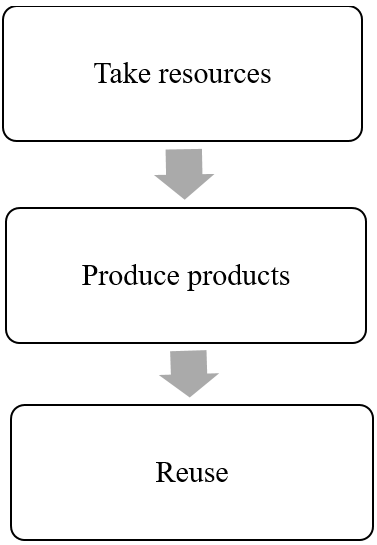
\includegraphics[width=0.3\textwidth]{media/gorn4/image4}
	\caption*{Fig.1 - Circular Economy Principle}
	\caption*{\normalfont\emph{Note: compiled by the authors}}
\end{figure}

In the context of the mining industry, the application of the circular
economy includes a number of key aspects:

One of the main principles of the circular economy in the mining
industry is the maximum recycling of materials, which includes the
development and implementation of waste processing technologies in order
to extract valuable materials for reuse in production processes.

The circular economy implies the efficient use of resources, which means
reducing losses during the extraction and processing of minerals.
Innovations in mining, enrichment and processing technologies are aimed
at maximizing the extraction of valuable components and minimizing
waste.

The principle of the circular economy includes the management of the
product life cycle - from resource extraction to end use. The principle
of the circular economy includes extending the service life of products,
facilitating their repair, upgrade and, ultimately, disposal with
minimal impact on the environment.

The use of monitoring technologies and feedback systems that allow for
continuous assessment and improvement of environmental and economic
indicators of production. This allows for a more effective response to
changes in processes and optimizes the use of resources.

Developing and implementing sustainable resource extraction methods that
minimise impacts on nature and include the use of technologies such as
zero-waste mining or processing methods and the introduction of
energy-efficient technologies.

Promoting circular ecosystems in which mining companies interact and
exchange resources and materials to maximise their reuse and minimise
waste {[}12{]}.

Encouraging innovation and research into technologies and methods that
support a circular economy in mining. This includes funding research
into improved processing technologies, resource efficiency and reduced
impacts {[}13{]}

A circular economy in mining not only contributes to environmental
sustainability, but can also be a key element in ensuring the long-term
sustainability of the industry and reducing negative environmental
impacts.

{\bfseries Materials and methods.} Based on the relevance and
socio-economic significance of this topic, especially in light of the
desire of the Republic of Kazakhstan to form a new scientific and
technological policy and aspirations for low-carbon development, we have
defined an integrated approach to the study, which includes not only
traditional methods of analysis and evaluation, but also the use of
advanced digitalization and automation technologies for a deeper
understanding and optimization of processes at the enterprise {[}14{]}.

The authors consider in detail each stage of the study, from the initial
collection of data to their analysis and interpretation. This approach
will identify potential areas for improving the efficiency and reducing
the cost of mining and transport operations and assess the environmental
aspects and carbon intensity of the technologies used. This approach is
important to ensure sustainable development of the mining industry and
its compliance with modern environmental standards and requirements.

Research question: The study is aimed at establishing a real
relationship between mining and transport and drilling and blasting
operations in the context of the efficiency of the geotechnological
complex of the Bakyrchy mining enterprise. Hypothesis put forward: The
hypothesis suggests that optimization of drilling and blasting and
mining and transport operations can significantly increase the
efficiency of geotechnological complexes, which in turn will improve the
profitability and environmental safety of field development.

Research stages. Research in the field of low-carbon development
strategy is important for achieving sustainable economic and
environmental growth. For successful implementation of such a strategy,
it is necessary to conduct a systematic scientific and practical study,
which would include a number of stages. The first stage is the analysis
of the relevance and socio-economic significance of the proposed
research in the context of the low-carbon development strategy of the
Republic of Kazakhstan. Then the object, subject, goals and objectives
of the study are determined. After this, the primary data on the current
situation at the enterprise is studied. Finally, new methods and
approaches for the analysis and optimization of processes are developed
and applied (Figure 2).
\end{multicols}

\begin{figure}[H]
	\centering
	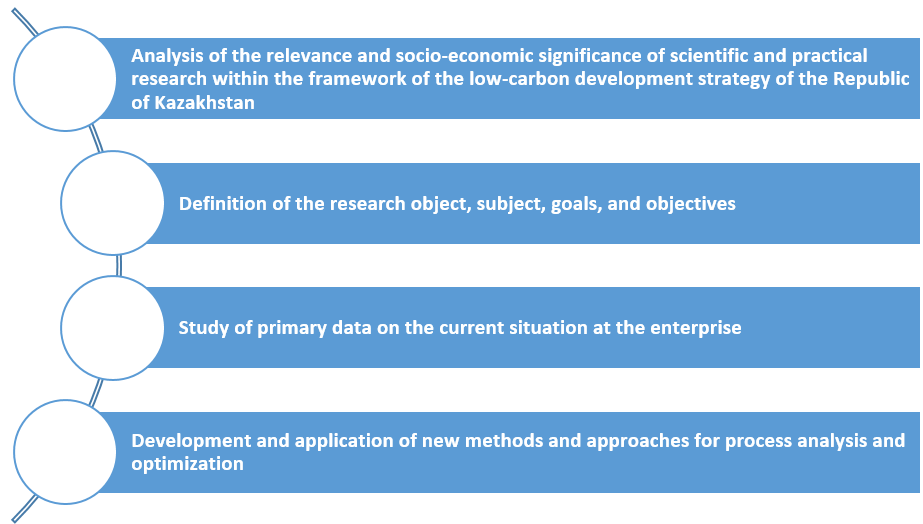
\includegraphics[width=0.75\textwidth]{media/gorn4/image5}
	\caption*{Fig.2 - Research stages}
	\caption*{\normalfont\emph{Note: compiled by the authors}}
\end{figure}

\begin{multicols}{2}
These stages represent a sequence of steps necessary to carry out a
successful study within the framework of a low-carbon development
strategy, thereby providing a basis for developing effective strategies
and solutions.

Research methods:

- Simulation modeling to assess various scenarios of mining and
transport and drilling and blasting operations.

- Technical and economic analysis to assess the efficiency and potential
for reducing the cost of work.

- Methods of digitalization and information analytical support for
process management and automation.

- Environmental audit to assess the carbon intensity and environmental
efficiency of technological processes {[}15{]}.

Research results:

- Proposal of specific measures to improve the efficiency of the
geotechnological complex.

- Analysis of the potential and directions for process optimization,
including assessment of the quality of the road surface, organization of
blasting operations, preparation of rocks and optimization of the
structure of intra-quarry rock flows.

- Development of methods for the environmental assessment of
geotechnological complexes in open-pit mining {[}16{]}.

The research is due to its relevance and socio-economic feasibility in
the context of modern tasks in the formation of a new scientific and
technological policy in the Republic of Kazakhstan, including aspects of
low-carbon economic development and modernization of the mining
industry.

One of the leading areas determining the efficiency of the mining
industry is the optimization of the fleet of the main mining and
transport equipment. Numerous studies and technical and technological
audits confirm the importance of this aspect not only in terms of
updating the model range and numerical ratio, but also in the context of
the constant emergence of new equipment modifications on the world
market. This observation emphasizes the need to adapt and modernize
equipment in accordance with current requirements and market trends
{[}17{]}.

Optimization of the depreciation policy of equipment, taking into
account its technical condition and service life. Adequate consideration
of these factors is often overlooked when planning mining and transport
complexes, which leads to significant discrepancies between the actual
and design efficiency of the equipment.

An important component of an integrated approach to managing mining
processes is the analysis of the quality of the road surface in quarry
areas. The quality of the road surface directly affects the speed modes
of transport, the time of trips of dump trucks and, as a result, the
overall productivity of the complex and the volume of environmental
emissions during the work. Particular attention is paid to the
optimization of drilling and blasting operations, especially when
developing hard rocks. The efficiency of organizing these operations
plays a key role in increasing the overall efficiency of the
geotechnical complex. Thoughtful planning and organization of drilling
and blasting operations contribute not only to increased productivity,
but also to reduced costs {[}18{]}.

{\bfseries Results and Discussions}. The research of the influence of the
quality of rock preparation for excavation and drilling and blasting
methods opens up new opportunities for increasing the overall efficiency
and reducing the cost of mining and transport operations. An important
factor here is the degree of loosening of rocks, which affects the
overall efficiency of the process.

The use of simulation modeling made it possible to evaluate various
scenarios for mining and transport and drilling and blasting operations,
which helps to improve the efficiency of these processes. Conducting a
technical and economic analysis made it possible to evaluate the
efficiency and potential for reducing the cost of work, which is an
important aspect when making management decisions. The use of
digitalization methods and information analytical support contributes to
the management and automation of processes in the mining industry, which
increases their efficiency. Conducting an environmental audit allows you
to assess the carbon intensity and environmental efficiency of
technological processes in the mining industry, which is important from
the point of view of compliance with environmental norms and standards.

The results of the research include proposals for specific measures to
improve the efficiency of the geotechnological complex, an analysis of
the potential and directions for optimizing processes, and the
development of methods for the environmental assessment of
geotechnological complexes in open pit mines.

An important area is the optimization of the organization of food for
drivers of mining and transport equipment, which, despite its seeming
secondary importance, has a significant impact on the productivity and
efficiency of the complex.

Optimization of the structure of intra-quarry rock flows and the
location of ore handling warehouses is also an important aspect that
allows increasing the efficiency of the geotechnological complex and
reducing costs.

The final stage is the development of methods for assessing the
environmental efficiency of the complexes, the introduction of digital
technologies and automation of management decisions, which helps to
increase the economic efficiency of the geotechnological complex and
reduce the costs of mining and transport operations, while improving the
profitability of deposit development {[}19{]}.

One of the important points in the economic assessment of the efficiency
of the geotechnological complex, as well as the impact of its work on
the efficiency of the enterprise as a whole. In this regard, it is
fundamentally important to establish the relationship between the main
economic indicators at the levels of the enterprise, quarry and the
geotechnological complex under consideration.

According to the presented data, the total cost of the enterprise is
102493545.67 tenge. Of these, the mining part accounts for 82260256.7
tenge or 80.26\% of the total volume. At the same time, with a given
volume of rock mass extracted at the quarry, the specific cost of m3 of
rock mass is 2481.3 tenge or \$ 5.45 (at the exchange rate of 1 US
dollar = 455 tenge). For the geotechnological complex, similar
indicators have values \hspace{0pt}\hspace{0pt}of 55,745,052.0 (54.3\%
of total costs) and 1,683.6 tenge/m3, respectively.

One of the main cost items for maintaining the functioning of the quarry
geotechnological complex are operating costs for the main mining and
transport equipment - depreciation charges and material costs. In this
regard, in the process of forming an economic and mathematical model of
the functioning of the geotechnological complex, take into account the
fact that the enterprise has established depreciation periods for the
main mining and transport equipment purchased in 2016 and later, in
particular dump trucks: BelAZ-75139 - 84 months and Komatsu HD785 - 60
months. The purchase prices of dump trucks are as follows: BelAZ 75139 -
594.2 million tenge (2021) and Komatsu HD785 - 410.7 million tenge
(2021). In 2016, 6 Komatsu HD 785-7 dump trucks were purchased, with a
service life of 60 months.

Another important item of operating costs taken into account is the
monthly salary of drivers and operators of the main process equipment.
Based on the adopted mode of organizing the main technological
processes, similar shift indicators are established, which participate
in the operational calculation of the cost of mining and transport
operations, based on the actual production volumes of the main product
of the functioning geotechnological complex. For 2023, according to the
enterprise, the salary of excavator drivers is set at 639,002.2 tenge /
month for drivers and 498,273.4 for assistant drivers. The salary of
dump truck drivers at the enterprise is set at 591,476.0 tenge for the
main workers and 532,377.0 for those who go on to replace them during
lunch breaks (Table 3).
\end{multicols}

\tcap{Table 3 - Calculation of costs for the extraction and processing of one m3 of rock mass for 2022-2023}
\begin{longtblr}[
  label = none,
  entry = none,
]{
  width = \linewidth,
  colspec = {Q[323]Q[142]Q[135]Q[92]Q[144]Q[98]},
  rows = {font = \footnotesize},
  row{1} = {c},
  row{2} = {c},
  column{4} = {c},
  column{6} = {c},
  cell{1}{1} = {r=2}{},
  cell{1}{2} = {r=2}{},
  cell{1}{3} = {c=2,r=2}{0.227\linewidth},
  cell{1}{5} = {c=2}{0.242\linewidth},
  cell{2}{5} = {c=2}{0.242\linewidth},
  cell{3}{2} = {c},
  cell{3}{3} = {c=2}{0.227\linewidth,c},
  cell{3}{5} = {c=2}{0.242\linewidth,c},
  cell{4}{2} = {c=5}{0.611\linewidth,c},
  cell{5}{2} = {c},
  cell{5}{3} = {c},
  cell{5}{5} = {c},
  cell{6}{2} = {c},
  cell{6}{3} = {c},
  cell{6}{5} = {c},
  cell{7}{2} = {c},
  cell{7}{3} = {c},
  cell{7}{5} = {c},
  cell{8}{2} = {c},
  cell{8}{3} = {c},
  cell{8}{5} = {c},
  cell{9}{2} = {c},
  cell{9}{3} = {c},
  cell{9}{5} = {c},
  cell{10}{2} = {c},
  cell{10}{3} = {c},
  cell{10}{5} = {c},
  cell{11}{2} = {c},
  cell{11}{3} = {c},
  cell{11}{5} = {c},
  cell{12}{2} = {c},
  cell{12}{3} = {c},
  cell{12}{5} = {c},
  cell{13}{2} = {c},
  cell{13}{3} = {c},
  cell{13}{5} = {c},
  cell{14}{2} = {c},
  cell{14}{3} = {c},
  cell{14}{5} = {c},
  cell{15}{2} = {c},
  cell{15}{3} = {c},
  cell{15}{5} = {c},
  cell{16}{2} = {c},
  cell{16}{3} = {c},
  cell{16}{5} = {c},
  cell{17}{2} = {c},
  cell{17}{3} = {c},
  cell{17}{5} = {c},
  cell{18}{2} = {c},
  cell{18}{3} = {c},
  cell{18}{5} = {c},
  cell{19}{2} = {c},
  cell{19}{3} = {c},
  cell{19}{5} = {c},
  cell{20}{2} = {c},
  cell{20}{3} = {c},
  cell{20}{5} = {c},
  cell{21}{2} = {c},
  cell{21}{3} = {c},
  cell{21}{5} = {c},
  cell{22}{2} = {c},
  cell{22}{3} = {c},
  cell{22}{5} = {c},
  cell{23}{2} = {c},
  cell{23}{3} = {c},
  cell{23}{5} = {c},
  cell{24}{2} = {c},
  cell{24}{3} = {c},
  cell{24}{5} = {c},
  cell{25}{2} = {c},
  cell{25}{3} = {c},
  cell{25}{5} = {c},
  cell{26}{2} = {c},
  cell{26}{3} = {c},
  cell{26}{5} = {c},
  cell{27}{2} = {c},
  cell{27}{3} = {c},
  cell{27}{5} = {c},
  cell{28}{2} = {c},
  cell{28}{3} = {c},
  cell{28}{5} = {c},
  cell{29}{2} = {c},
  cell{29}{3} = {c},
  cell{29}{5} = {c},
  cell{30}{2} = {c},
  cell{30}{3} = {c},
  cell{30}{5} = {c},
  cell{31}{2} = {c},
  cell{31}{3} = {c},
  cell{31}{5} = {c},
  vlines,
  hline{1,3-32} = {-}{},
  hline{2} = {5-6}{},
}
{
			Name
			of works and expenses
			\\~\\~} & Cost
			Amount. & Mining
			Part &  & Geotechnological
			complex & \\
 &  &  &  & Fact & \\
Share
			in total cost, \% & 100\% & 80,25\% &  & 54,39\% & \\
Volume
			of rock mass, thousand m3. & \textbf{2022			г.			-33			111,			87			/2023			г.			–			30770,0} &  &  &  & \\
Total
			wages of workers, thousand tenge & 7
			946
			581,0 & 5
			221
			194,0 & 157,7 & 5
			221
			194,0 & 157,7\\
Depreciation,
			thousand tenge. & 24
			154 670,1 & 19
			494 675,7 & 588,8 & 19
			494 675,7 & 588,8\\
Materials,
			thousand tenge & 805
			559,3 & 750
			617,6 & 22,7 & 750
			617,6 & 22,7\\
Fuels
			and lubricants & 13
			155 053,3 & 12
			405 334,7 & 374,6 & 16
			330 487,6 & 493,2\\
Energy
			tenge/kW. & 2
			031
			750,7 & 438
			098,9 & 13,2 & 438
			098,9 & 13,2\\
rent & 216
			022,0 & 211
			427,8 & 6,4 & {~\\~} & {~\\~}\\
spare
			parts & 12
			065 947,7 & 4
			164
			599,5 & 125,8 & 17
			450,1 & 0,5\\
travel
			expenses & 21
			638,4 & 14
			448,8 & 0,4 & {~\\~} & {~\\~}\\
utilities & 250
			845,1 & 172
			056,6 & 5,2 & {~\\~} & {~\\~}\\
Taxes
			(fee for emissions) & 1
			301
			628,5 & 1
			152
			575,0 & 34,8 & 1
			152
			575,0 & 34,8\\
Occupational
			safety & 90
			554,3 & 87
			226,3 & 2,6 & {~\\~} & {~\\~}\\
Food & 638
			543,9 & 397
			603,2 & 12,0 & {~\\~} & {~\\~}\\
{
			Other
			(unaccounted for + personnel\\delivery)
		} & 326
			812,4 & 243
			241,1 & 7,3 & 243
			241,1 & 7,3\\
Sn & 453
			281,7 & 303
			186,8 & 9,2 & 303
			186,8 & 9,2\\
So & 187
			067,9 & 118
			795,8 & 3,6 & 118
			795,8 & 3,6\\
OSMS
			+ OPPV & 472
			324,6 & 327
			115,8 & 6,9 & 327
			115,8 & 9,9\\
MET & 16
			418 696,0 & 16
			417 273,3 & 495,8 & {~\\~} & {~\\~}\\
Tires,
			thousand tenge & {~\\~} & {~\\~} & {~\\~} & 6419071,8 & 193,9\\
Repair
			and service & 5
			531
			716,9 & 4
			300
			606,7 & 129,9 & 4
			928
			541,8 & 148,8\\
Services & 39
			244,1 & 37
			891,1 & 1,1 & {~\\~} & {~\\~}\\
Contractor
			(drilling and blasting operations) & 14
			966 230,8 & 14
			966 195,8 & 452,0 & {~\\~} & {~\\~}\\
Training & 27
			918,5 & 17
			985,7 & 0,5 & {~\\~} & {~\\~}\\
Insurance & 286
			707,2 & 189
			192,2 & 5,7 & {~\\~} & {~\\~}\\
Expert
			and analytical services & 342
			910,1 & 286
			273,6 & 8,6 & {~\\~} & {~\\~}\\
Transport
			services & 761
			844,5 & 542
			625,9 & 16,4 & {~\\~} & {~\\~}\\
TOTAL
			expenses tenge & \textbf{102			493			548,7} & \textbf{82			260			256,7} & \textbf{2			481,3} & \textbf{55			745			052,0} & \textbf{1			683,6}\\
Dollar
			(at the rate of \$1 = 455 tenge) & {~\\~} & {~\\~} & \textbf{5,45} & {~\\~} & \textbf{3,70}
\end{longtblr}

\begin{multicols}{2}
General practice and experience in researching the efficiency of quarry
geotechnological complexes, traditionally, areas related to compliance
with the depreciation policy in relation to dump trucks and optimization
of their loading mode, by optimizing the equipment replacement schedule
and maintaining the workshop profitability of the mining and transport
complex at an optimal level, have significant potential in this regard.
In this case, due to the insignificance of the term of open-pit mining,
this direction can be implemented only in a small part of the existing
total potential. A full-fledged economic assessment of the efficiency of
the geotechnological complex from the quality of rock preparation for
extraction at the stage of drilling and blasting operations requires
adequate consideration of the corresponding change in the traction
forces of excavators during the process of rock extraction with
subsequent reliable identification of energy costs, as well as the
corresponding volumes of costs for drilling and blasting operations. In
this direction, additional studies are also required with the
corresponding variation in the volumes of buckets and dump truck bodies.

The most valuable thing in conducting a set of researches is identifying
the economic effect realized by the enterprise from the deviation from
the design solution adopted at the enterprise for opening the quarry and
organizing the transportation of overburden rock mass to the dump. This
economic effect is about 6263.60 million tenge per year with a
significant decrease in the indicator of optimal productivity of the
geotechnological complex {[}20{]}.

Analysis of other economic effects shows that the greatest potential for
reducing the cost of mining and transport operations in the established
mining-technical, mining-geometric, mining-geological, organizational
and economic conditions are in the areas of improving the quality of the
road surface of intra-quarry roads, as well as optimizing the structure
and number of the listed fleet of the main technological equipment.
\end{multicols}

\tcap{Table 2 - Potential economic effect, thousand tenge per year}
\begin{longtblr}[
  label = none,
  entry = none,
]{
  width = \linewidth,
  colspec = {Q[560]Q[381]},
  row{1} = {c},
  cell{4}{1} = {c=2}{0.941\linewidth},
  hlines,
  vlines,
}
\textbf{Optimization			direction} & \textbf{Potential			economic effect (thousand tenge per year)}\\
Improving
			the quality of road surfaces of quarry roads & Approximately
			1268.27\\
Optimization
			of the structure and number of the list of the main technological
			equipment & Approximately
			1035.42\\
Note:
			compiled by the authors & 
\end{longtblr}

\begin{multicols}{2}
The total potential economic effect is about 1268.27 thousand tenge per
year. Taking into account the lack of practical possibility of replacing
the diesel fleet of excavators with electric ones with the corresponding
technological parameters, the real potential for obtaining an economic
effect will be 1035.42 million tenge per year.

{\bfseries Conclusion}. The conducted research considered the efficiency of
the quarry geotechnological complex with varying various factors of
mining engineering, mining-geometric, mining-geological, organizational
and economic nature.

In the course of research using the method of simulation
logical-statistical and object-oriented modeling, the current state and
economic efficiency of the functioning of the Bakyrchik quarry
geotechnological complex were analyzed and assessed with a set of
studies of its operation under various qualitative characteristics of
the extracted rock mass.

As a result of the work carried out, the dependences of the economic
efficiency of the geotechnological complex on the preparation of rocks
for excavation were determined; the potential for increasing efficiency
and directions for its implementation with the development of a set of
appropriate measures were determined; software and methodological
support for the formation of digital twins of quarry geotechnological
complexes were improved using the simulation modeling method; directions
were determined and a set of specific measures were developed to
increase efficiency and reduce the cost of mining and transport
operations in the Bakyrchik quarry of Bykyrchik Mining Enterprise LLP.

The maximum possible planned productivity of the quarry geotechnological
complex in terms of rock mass is ensured by the high organization of
mining and transport operations, high-quality operational management of
the involved mining and transport equipment. The identified potential
for increasing the efficiency of the geotechnological complex and
reducing the cost of mining and transport operations is associated with
the use of a process approach in management and can be most effectively
implemented with the appropriate adaptation of the automated management
system for mining and transport operations used in the quarry, providing
operational accounting and operational economic assessment of the
operation of elements and subsystems of the quarry geotechnological
system. It is advisable to implement modules for monitoring the loading
of sections of the quarry motor transport system, operational accounting
and control of environmental emissions and dust in the quarry space, and
the introduction of a dynamic approach to accounting and control of
energy consumption by motor transport.

The conclusions and proposals resulting from the conducted research work
may be of interest to a wide range of specialists and managers of the
enterprise on technical and mining-production issues, on digital
transformations and automated control systems, the energy service and
the environmental protection department, as well as specialists in the
planning and economic direction in terms of the formation of the economy
of process management at the enterprise.
\end{multicols}

\begin{center}
{\bfseries References}
\end{center}

\begin{references}
1. Naugol' nova I.A. Processnyj podhod k upravleniju:
jevoljucija, sovremennye vyzovy, innovacii // Kreativnaja jekonomika.-
2023.-Т.17(6).- S.2143--2164. DOI 10.18334/ce.17.6.117951{[}in
Russian{]}.

2. Kaplan A.V., Galiev S.Zh. Processnoe upravlenie gornotransportnym
kompleksom v kar' ere na osnove jekonomicheskih
kriteriev // Gornyj zhurnal.-2017.- № 6.- S.28--32.
DOI 10.17580/gzh.2017.06.05 {[}in Russian{]}.

3. McCoy J.T., Auret L. Machine learning applications in minerals
processing: A review // Minerals Engineering.- 2019.- Vol.132.- P.
95-109. DOI
\href{https://doi.org/10.1016/j.mineng.2018.12.004}{10.1016/j.mineng.2018.12.004}.

4. Ayoub R., Baïna S., Mhada F.Z., El Bachari E. Predictive maintenance
in mining industry: Grinding mill case study // Procedia Computer
Science.-2022.-Vol.207.-P.2483--2492.DOI
\href{https://doi.org/10.1016/j.procs.2022.09.306}{10.1016/j.procs.2022.09.306}.

5. Salem K., AbdelGwad E., Kouta H. Predicting forced blower failures
using machine learning algorithms and vibration data for effective
maintenance strategies // Journal of Failure Analysis and
Prevention.-2023.-Vol.23.- P.2191--2203. DOI
\href{http://dx.doi.org/10.1007/s11668-023-01765-x}{10.1007/s11668-023-01765-x}.

6. \href{https://www.researchgate.net/profile/Oscar-Restrepo-6?_tp=eyJjb250ZXh0Ijp7ImZpcnN0UGFnZSI6InB1YmxpY2F0aW9uIiwicGFnZSI6InB1YmxpY2F0aW9uIn19}{Restrepo}
O. Exploring new sustainable horizons in the mining industry: Circular
economy, sustainability, and technological development // Material
Science Research India.-2024.- Vol.21(2). - P.72-73. DOI
\href{http://dx.doi.org/10.13005/msri/210202}{10.13005/msri/210202}.

7. Gilligan R., Aleksandar N. The extraction of vanadium from
titanomagnetites and other sources // Minerals Engineering. - 2020.
-Vol.146. -P.106. DOI
\href{https://doi.org/10.1016/j.mineng.2019.106106}{10.1016/j.mineng.2019.106106}.

8. Ghorbani B., Saharkhiz M., Li J. A novel integrated system for
sustainable generation of hydrogen and liquid hydrocarbon fuels using
the five-step ZnSI thermochemical cycle, biogas upgrading process, and
solar collectors//Journal of Cleaner Production.-2021.-Vol.312. DOI
\href{https://doi.org/10.1016/j.jclepro.2021.127715}{10.1016/j.jclepro.2021.127715}.

9. Koyama K., Krane J. Energy security through FDI: The legacy of Early
Japanese Investment in the Oil Sectors of the Persian Gulf //
Resources Policy.-2021.-Vol.74:102165. DOI\\
\href{https://doi.org/10.1016/j.resourpol.2021.102165}{10.1016/j.resourpol.2021.102165}.
2021.

10. Mutani G., Todeschi V., Beltramino S. Energy Consumption Models at
Urban Scale to Measure Energy Resilience //~Sustainability. - 2020. -
Vol.12.- № 14. DOI
\href{https://doi.org/10.3390/su12145678}{10.3390/su12145678}.

11. Khammar M., Zhu Y., Xu Y. Centrifugal recovery of solvent-diluted
bitumen from oil sands // Minerals Engineering. - 2019. - Vol.136. --
P.8-17. DOI
\href{https://doi.org/10.1016/j.mineng.2019.03.005}{10.1016/j.mineng.2019.03.005}.

12. Munagala V., Thudumu S., Logothetis I., Bhandari S., Vasa R., Mouzakis
K. A comprehensive survey on machine learning applications for
drilling and blasting in surface mining // Machine Learning with
Applications. - 2024. - Vol.15. DOI 10.1016/j.mlwa.2023.100517.

13. Kaplan A. V. Upravlenie social' no-jekonomicheskim
razvitiem gornodobyvajushhego predprijatija.-M.: Jekonomika, 2015. -
270 s. ISBN 978-5-282-03409-7~ {[}in Russian{]}.

14. Galiev S.Zh., Samenov G.K. Avtomatizirovannaja sistema korporativnogo
upravlenija \\geotehnologicheskim kompleksom/ Sbornik dokladov i katalog
VII Mezhotraslevoj konferencii \\«Avtomatizacija proizvodstva -
2016»,-M.-2016.-S.38-41 URL:
\href{https://official.satbayev.university/download/document/42896/МАГ_2024}{https://official.satbayev.university}
Data obrashhenija: 05.02.25). {[}in Russian{]}.

15. Galiev S.Zh., Galiev D.A., Sejtaev E.N., Uteshov E.N. O edinoj
metodologii upravlenija \\geotehnologicheskim kompleksom na otkrytyh
gornyh rabotah/ Gornyj zhurnal.- 2019.- №12 S.70-75. DOI
10.17580/gzh.2019.12.15. {[}in Russian{]}.

16. Rakishev B.R., Shubin I.L., Alenichev I.A. i dr. Snizhenie
poter'{} i razubozhivanija pri otrabotke rudnyh blokov
slozhnoj konfiguracii i bol' shoj doli malomoshhnyh
rudnyh tel. /Otchjot o nauchno-issledovatel' skoj rabote
TOO «Qazaqstan Smart Technology» ot 27.12.2022 g. Almaty.: 2023.-41s.
IRN123PKH003. URL:
\url{https://official.satbayev.university/download/document/42896/МАГ_2024}
.- Data obrashhenija: \\05.02.25). {[}in Russian{]}.

17. Galiyev S.Zh., Samenov G.K., Zhusupov K.K., Galiyev D.A. Conception
of automated management of geotechnological complex on an innovative
base / 24th World Mining Congress Proceedings / Innovation / Instituto
Brasileiro de Mineracio. IBRAM. - 2016. - 2555p.

18. Galiev D.A., Uteshov E.T., Tekenova А.Т. Digitalization of
Technological and Organizational Processes in Mining Operations through
the Implementation of a Key Performance Indicators Installation and\\
Monitoring System // Bulletin of the National Academy of Sciences of the
Republic of Kazakhstan. Series of Geology and Technical Sciences.-
2020. - Vol.5 (443).- P.47-53. DOI 10.32014/2020.2518-170x.103

19. Zarubin M., Statsenko L., Spiridonov P., Zarubina V., Melkumyan N.,
Salykova O.GIS Module for Environmental Impact Assessment of Open-Pit
Mining Projects for Small-Scale Mining Operators in Kazakhstan //
Sustainability. - 2021. - Vol.13(12): 6971. DOI 10.3390/su13126971.
\end{references}

\begin{authorinfo}
\emph{{\bfseries Сведения об авторах}}

Галиев Д.А.- доктор PhD, директор ТОО «Qazaqstan smart technology»,
Астана, Казахстан, e-mail:
\href{mailto:info@qstechnology.kz}{\nolinkurl{info@qstechnology.kz}};

Малдынова А.В.- доктор PhD, доцент, Университет Международного Бизнеса
им. К. Сагадиева, Алматы, Казахстан, e-mail:
\href{mailto:maldynova.a@uib.kz}{\nolinkurl{maldynova.a@uib.kz}}.


\emph{{\bfseries Information about the authors}}

Galiyev D.A. - doctor PhD, Director of Qazaqstan smart technology LLP,
Astana, Kazakhstan, e-mail:
\href{mailto:info@qstechnology.kz}{\nolinkurl{info@qstechnology.kz}};

Maldynova A.V.- doctor PhD, Associate Professor, Kenzhegali Sagadiyev
University of International Business Almaty, \\Kazakhstan, e-mail:
\href{mailto:maldynova.a@uib.kz}{\nolinkurl{maldynova.a@uib.kz}}.
\end{authorinfo}
